\item \points{40} {\bf Linear Classifiers (logistic regression and GDA)}

In this problem, we cover two probabilistic linear classifiers we have
covered in class so far. First, a discriminative linear classifier: logistic
regression. Second, a generative linear classifier: Gaussian discriminant
analysis (GDA). Both the algorithms find a linear decision boundary that
separates the data into two classes, but make different assumptions. Our goal
in this problem is to get a deeper understanding of the similarities and
differences (and, strengths and weaknesses) of these two algorithms.

For this problem, we will consider two datasets, along with starter codes provided in the following
files:
\begin{center}
\begin{itemize} %[label=\roman*.]
	\item \url{src/linearclass/ds1_{train,valid}.csv}
	\item \url{src/linearclass/ds2_{train,valid}.csv}
        \item \url{src/linearclass/logreg.py}
        \item \url{src/linearclass/gda.py}
\end{itemize}
\end{center}
Each file contains $\nexp$ examples, one example $(x^{(i)}, y^{(i)})$ per row.
In particular, the $i$-th row contains columns $x^{(i)}_1\in\Re$,
$x^{(i)}_2\in\Re$, and $y^{(i)}\in\{0, 1\}$. In the subproblems that follow, we
will investigate using logistic regression and Gaussian discriminant analysis
(GDA) to perform binary classification on these two datasets.

\begin{enumerate}
	\item \subquestionpoints{10}

%\textbf{TBD RETIRE THIS QUESTION? Q4c is a more generic version of this}

In lecture we saw the average empirical loss for logistic regression:
\begin{equation*}
	J(\theta)
	= -\frac{1}{\nexp} \sum_{i=1}^\nexp \left(y^{(i)}\log(h_{\theta}(x^{(i)}))
		+  (1 - y^{(i)})\log(1 - h_{\theta}(x^{(i)}))\right),
\end{equation*}
where $y^{(i)} \in \{0, 1\}$, $h_\theta(x) = g(\theta^T x)$ and
$g(z) = 1 / (1 + e^{-z})$.

Find the Hessian $H$ of this function, and show that for any vector $z$, it
holds true that
%
\begin{equation*}
    z^T H z \ge 0.
\end{equation*}
%
{\bf Hint:} You may want to start by showing that
$\sum_i\sum_j z_i x_i x_j z_j = (x^Tz)^2 \geq 0$. Recall also that
$g'(z) = g(z)(1-g(z))$.

{\bf Remark:} This is one of the standard ways of showing that the matrix $H$
is positive semi-definite, written ``$H \succeq 0$.''  This implies that $J$ is
convex, and has no local minima other than the global one. If you have some
other way of showing $H \succeq 0$, you're also welcome to use your method
instead of the one above.


        \ifnum\solutions=1 {
            \begin{answer}
	Your solution here.
\end{answer}

        } \fi

	\item \subquestionpoints{5} \textbf{Coding problem.}
Follow the instructions in \texttt{src/linearclass/logreg.py} to train a
logistic regression classifier using Newton's Method.
Starting with $\theta = \vec{0}$, run Newton's Method until the updates to
$\theta$ are small: Specifically,  train until the first iteration $k$ such
that $\|\theta_{k} - \theta_{k-1}\|_1 < \epsilon$, where
$\epsilon = 1\times 10^{-5}$. Make sure to write your model's predicted probabilities on
the validation set to the file specified in the code.

Include a plot of the \textbf{validation data} with $x_1$ on the horizontal axis and $x_2$ on the vertical axis.
To visualize the two classes, use a different symbol for examples $x^{(i)}$
with $y^{(i)} = 0$ than for those with $y^{(i)} = 1$. On the same figure, plot the decision boundary
found by logistic regression (i.e, line corresponding to $p(y|x) = 0.5$).


        \ifnum\solutions=1 {
            \begin{answer}
	\begin{figure}[H]
		\centering
		\vspace{2mm}
		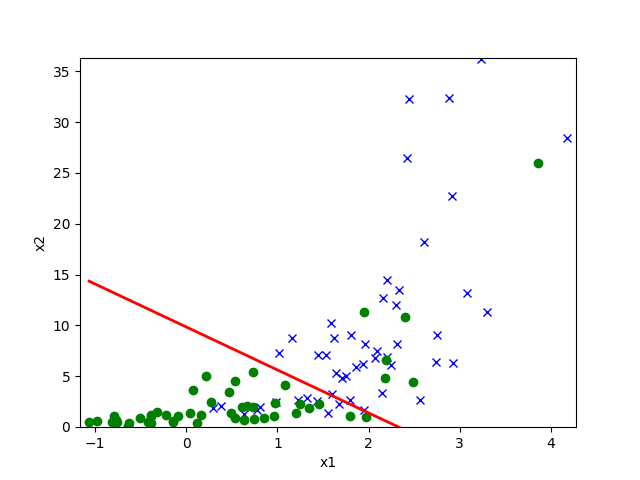
\includegraphics[width=0.65\linewidth]{../src/linearclass/logreg_pred_1.png}
        \caption{Separating hyperplane for logistic regression on Dataset 1}
	\end{figure}

\end{answer}

        } \fi


	\item \subquestionpoints{5}
Recall that in GDA we model the joint distribution of $(x, y)$ by the following
equations:
%
\begin{eqnarray*}
	p(y) &=& \begin{cases}
	\phi & \mbox{if~} y = 1 \\
	1 - \phi & \mbox{if~} y = 0 \end{cases} \\
	p(x | y=0) &=& \frac{1}{(2\pi)^{\di/2} |\Sigma|^{1/2}}
		\exp\left(-\frac{1}{2}(x-\mu_{0})^T \Sigma^{-1} (x-\mu_{0})\right) \\
	p(x | y=1) &=& \frac{1}{(2\pi)^{\di/2} |\Sigma|^{1/2}}
		\exp\left(-\frac{1}{2}(x-\mu_1)^T \Sigma^{-1} (x-\mu_1) \right),
\end{eqnarray*}
%
where $\phi$, $\mu_0$, $\mu_1$, and $\Sigma$ are the parameters of our model.

Suppose we have already fit $\phi$, $\mu_0$, $\mu_1$, and $\Sigma$, and now
want to predict $y$ given a new point $x$. To show that GDA results in a
classifier that has a linear decision boundary, show the posterior distribution
can be written as
%
\begin{equation*}
	p(y = 1\mid x; \phi, \mu_0, \mu_1, \Sigma)
	= \frac{1}{1 + \exp(-(\theta^T x + \theta_0))},
\end{equation*}
%
where $\theta\in\Re^\di$ and $\theta_{0}\in\Re$ are appropriate functions of
$\phi$, $\Sigma$, $\mu_0$, and $\mu_1$.


        \ifnum\solutions=1 {
            \begin{answer}
	For shorthand, we let $\mc{H} = \{\phi, \Sigma, \mu_{0}, \mu_1\}$ denote
	the parameters for the problem.
	Since the given formulae are conditioned on $y$, use Bayes rule to get:
	\begin{align*}
		p(y =1| x ; \phi, & \Sigma, \mu_{0}, \mu_1)\\
		& = \frac {p(x|y=1; \phi, \Sigma, \mu_{0}, \mu_1) p(y=1; \phi, \Sigma,
			\mu_{0}, \mu_1)} {p(x; \phi, \Sigma, \mu_{0}, \mu_1)}
			\notag\\
		& = \frac {p(x|y=1; \mc{H}) p(y=1; \mc{H})}
			{p(x|y=1; \mc{H}) p(y=1; \mc{H}) + p(x|y={0}; \mc{H}) p(y={0};
			\mc{H})}\notag\\
		&= \frac{\exp\left(-\frac{1}{2} (x-\mu_1)^T \Sigma^{-1} (x-\mu_1) \right)
			\phi}
			{\exp\left(-\frac{1}{2} (x-\mu_1)^T \Sigma^{-1} (x-\mu_1) \right)
			\phi + \exp\left(-\frac{1}{2} (x-\mu_{0})^T \Sigma^{-1} (x-\mu_{0}) \right)
			(1-\phi)}\notag\\
		&= \frac{1} {1+ \frac{1-\phi}{\phi}
			\exp\left(-\frac{1}{2} (x-\mu_{0})^T \Sigma^{-1} (x-\mu_{0}) + \frac{1}{2}
			(x-\mu_1)^T \Sigma^{-1} (x-\mu_1)\right)}\notag\\
		&= \frac{1} {1 +\exp\left(\log(\frac{1-\phi}{\phi}) -
			\frac{1}{2}(x-\mu_{0})^T \Sigma^{-1} (x-\mu_{0}) + \frac{1}{2}(x-\mu_1)^T
			\Sigma^{-1} (x-\mu_1)\right)}.
	\end{align*}
	Now, we expand and rearrange the difference of quadratic terms
	in the preceding expression, finding that
	\begin{align*}
		\lefteqn{(x-\mu_{0})^T \Sigma^{-1} (x-\mu_{0}) - (x-\mu_1)^T
		\Sigma^{-1} (x-\mu_1)} \\
		& =  x^T \Sigma^{-1} x - \mu_{0}^T\Sigma^{-1} x -
			x^T\Sigma^{-1}\mu_{0} + \mu_{0}^T \Sigma^{-1} \mu_{0} - x^T \Sigma^{-1} x +
			\mu_1^T \Sigma^{-1} x + x^T\Sigma^{-1}\mu_1 - \mu_1^T \Sigma^{-1}
			\mu_1 \\
		& = - 2 \mu_{0}^T\Sigma^{-1} x
			+ \mu_{0}^T \Sigma^{-1} \mu_{0} + 2 \mu_1^T \Sigma^{-1} x
			- \mu_1^T \Sigma^{-1}\mu_1 \\
		& = 2 (\mu_1 - \mu_{0})^T \Sigma^{-1} x + \mu_{0}^T \Sigma^{-1} \mu_{0}
			- \mu_1^T \Sigma^{-1} \mu_1.
	\end{align*}
	Thus, we have
	\begin{equation*}
		p(y = 1 \mid x; \mc{H})
		= \frac{1}{1 + \exp\left(\log \frac{1 - \phi}{\phi}
		+ \half \mu_1^T \Sigma^{-1} \mu_1 - \half \mu_{0}^T \Sigma^{-1} \mu_{0}
		+ (\mu_{0} - \mu_1)^T \Sigma^{-1} x \right)}.
	\end{equation*}
	and setting
	\begin{equation*}
		\theta = -\Sigma^{-1}(\mu_{0} - \mu_1)
			~~ \mbox{and} ~~ \theta_0 = \half (\mu_{0}^T \Sigma^{-1} \mu_{0}
			- \mu_1^T \Sigma^{-1} \mu_1) - \log \frac{1 - \phi}{\phi}
	\end{equation*}
	gives that
	\begin{equation*}
	p(y = 1 \mid x; \phi, \Sigma, \mu_{0}, \mu_1)
	= \frac{1}{1 + \exp(-(\theta^T x + \theta_0))}.
	\end{equation*}
\end{answer}

        }\fi

	\item \subquestionpoints{7} Given the dataset, we claim that the maximum
  likelihood estimates of the parameters are given by
  \begin{eqnarray*}
    \phi &=& \frac{1}{\nexp} \sum_{i=1}^\nexp 1\{y^{(i)} = 1\} \\
\mu_{0} &=& \frac{\sum_{i=1}^\nexp 1\{y^{(i)} = {0}\} x^{(i)}}{\sum_{i=1}^\nexp
1\{y^{(i)} = {0}\}} \\
\mu_1 &=& \frac{\sum_{i=1}^\nexp 1\{y^{(i)} = 1\} x^{(i)}}{\sum_{i=1}^\nexp 1\{y^{(i)}
= 1\}} \\
\Sigma &=& \frac{1}{\nexp} \sum_{i=1}^\nexp (x^{(i)} - \mu_{y^{(i)}}) (x^{(i)} -
\mu_{y^{(i)}})^T
  \end{eqnarray*}
  The log-likelihood of the data is
  \begin{eqnarray*}
\ell(\phi, \mu_{0}, \mu_1, \Sigma) &=& \log \prod_{i=1}^\nexp p(x^{(i)} , y^{(i)};
\phi, \mu_{0}, \mu_1, \Sigma) \\
&=& \log \prod_{i=1}^\nexp p(x^{(i)} | y^{(i)}; \mu_{0}, \mu_1, \Sigma) p(y^{(i)};
\phi).
  \end{eqnarray*}
By maximizing $\ell$ with respect to the four parameters,
prove that the maximum likelihood estimates of $\phi$, $\mu_{0}, \mu_1$, and
$\Sigma$ are indeed as given in the formulas above.  (You may assume that there
is at least one positive and one negative example, so that the denominators in
the definitions of $\mu_{0}$ and $\mu_1$ above are non-zero.)


        \ifnum\solutions=1 {
            \begin{answer}
we will find maximum parameters of log likelihood by searching $\nabla l = 0$ for each parameter. 

  \begin{equation*}
      l(\phi,\mu_0, \mu_1, \Sigma) 
      = \sum_{i=1}^\nexp(log(p(x^{i}|y^{i}) + \sum_{i=1}^\nexp(log(p(y^{i})))
  \end{equation*}
  
  \begin{equation*}
      p(y^{i}) = \phi^{y^{i}}(1-\phi)^{y^{i}}
\end{equation*}
\begin{equation*}
      p(x^{i}|y^{i}) = \frac{1}{(2\pi)^{0.5d}|\Sigma|^{0.5}}exp(-0.5(x-\mu_(y^{i}))^{T}\Sigma^{-1}(x-\mu_(y^{i})))
 \end{equation*}
 
 \begin{equation*}
     \nabla_\phi l = 0 = \nabla_\phi \sum_{i=1}^\nexp(log(p(x^{i}|y^{i}) + \nabla_\phi\sum_{i=1}^\nexp(log(p(y^{i}))) = 
\end{equation*}
\begin{equation*}
      \nabla_\phi\sum_{i=1}^\nexp(log(\frac{1}{(2\pi)^{0.5d}|\Sigma|^{0.5}}exp(-0.5(x-\mu_(y^{i}))^{T}\Sigma^{-1}(x-\mu_(y^{i})))) + \nabla_\phi \sum_{i=1}^\nexp log(\phi^{y^{i}}(1-\phi)^{y^{i}}) = 
 \end{equation*} 
 \begin{equation*}
     0 + \sum_{i=1}^\nexp (\frac{y^{i}}{\phi} - \frac{1-y^{i}}{1-\phi}) = 0
 \end{equation*}
 \begin{equation*}
     \sum_{i=1}^\nexp (\frac{y^{i}}{\phi}) = \sum_{i=1}^\nexp( \frac{1-y^{i}}{1-\phi}) \Rightarrow \frac{1}{\phi}\sum_{i=1}^\nexp y^{i} = \frac{1}{1-\phi}(n - \sum_{i=1}^\nexp y^{i}) 
 \end{equation*}
 
 If we denote $\sum_{i=1}^\nexp y^{i}$ as X for the convenience of calculation, we get
 \begin{equation*}
     \frac{x}{\phi} = \frac{n-X}{1-\phi} \Rightarrow X-X\phi = n\phi - X\phi
 \end{equation*}
 Thus
 \begin{equation*}
     \phi = \frac{X}{n} = \frac{1}{n}\sum_{i=1}^\nexp y^{i} =  \frac{1}{n}\sum_{i=1}^\nexp 1\{y^{(i)} = 1\} \\
 \end{equation*}
 
For finding maximum $\mu_y$ for the likelihood function, we need to use $\nabla_\mu_y l = 0$.

First, 
\begin{equation*}
    l = \sum_{i=1}^\nexp(log(p(x^{i}|y^{i})) + \sum_{i=1}^\nexp log(p(y^{i}) = 
\end{equation*}
\begin{equation*}
\sum_{i=1}^\nexp(log(\frac{1}{(2\pi)^{0.5d}|\Sigma|^{0.5}}exp(-0.5(x-\mu_(y^{i}))^{T}\Sigma^{-1}(x-\mu_(y^{i})))) + \sum_{i=1}^\nexp log(\phi^{y^{i}}(1-\phi)^{y^{i}})
\end{equation*}
 \begin{equation*}
     \nabla_\mu_y\sum_{i=1}^\nexp(log(\frac{1}{(2\pi)^{0.5d}|\Sigma|^{0.5}}exp(-0.5(x-\mu_(y^{i}))^{T}\Sigma^{-1}(x-\mu_(y^{i})))) + \nabla_\mu_y \sum_{i=1}^\nexp log(\phi^{y^{i}}(1-\phi)^{y^{i}})
 \end{equation*}
 \begin{equation*}
     0 = \nabla_\mu_y\sum_{i=1}^\nexp (-0.5(x-\mu_y)^{T}\Sigma^{-1}(x-\mu_y)) + 0
 \end{equation*}
\begin{equation*}
    -0.5 *\nabla_\mu_y\sum_{i=1}^\nexp (x^{T}\Sigma^{-1}x-x^{T}\Sigma^{-1}\mu_y - \mu_y^{T}\Sigma^{-1}x + \mu_y^{T}\Sigma^{-1}\mu_y) = 
\end{equation*}
\begin{equation*}
    -0.5*\nabla_\mu_y\sum_{i=1}^\nexp(x^{T}\Sigma^{-1}x- 2\mu_y^{T}\Sigma^{-1}x + \mu_y^{T}\Sigma^{-1}\mu_y) = 
\end{equation*}
 (Since $\mu_y^{T}\Sigma^{-1}x$ is 1x1 matrix, it is equivalent with its transpose $x^{T}\Sigma^{-1}\mu_y$.)
 \begin{equation*}
     \sum_{i=1}^\nexp(\Sigma^{-1}x - \Sigma^{-1}\mu_y) = 0
     \Rightarrow \Sigma \sum_{i=1}^\nexp(\Sigma^{-1}x - \Sigma^{-1}\mu_y) = \sum_{i=1}^\nexp(x - \mu_y) = 0
 \end{equation*}
 Thus,
 \begin{equation*}
     \sum_{i=1}^\nexp x = \sum_{i=1}^\nexp \mu_y
 \end{equation*}
 
 Since $\mu_y$ has different values depending on the y values, we will use indicator function in order to erase the other values which are not relevant to current y value. 
 \begin{equation*}
     \sum_{i=1}^\nexp 1\{y^{(i)} = k\} \\x^{i} = \sum_{i=1}^\nexp 1\{y^{(i)} = k\} \\\mu_y 
 \end{equation*}
 (k = 0 or 1)
 
 
 So, $\mu_y$ is...
 \begin{equation*}
     \frac{\sum_{i=1}^\nexp 1\{y^{(i)} = k\} \\x^{i}}{\sum_{i=1}^\nexp 1\{y^{(i)} = k\} \\} 
 \end{equation*}
 (k = 0 or 1)
 
 From the equation above we can know...
 \begin{equation*}
     \mu_0 = \frac{\sum_{i=1}^\nexp 1\{y^{(i)} = 0\} \\x^{i}}{\sum_{i=1}^\nexp 1\{y^{(i)} = 0\} \\} 
 \end{equation*}
 \begin{equation*}
     \mu_1 = \frac{\sum_{i=1}^\nexp 1\{y^{(i)} = 1\} \\x^{i}}{\sum_{i=1}^\nexp 1\{y^{(i)} = 1\} \\} 
 \end{equation*}
 
 Finally, in order to find the maximum likelihood estimate of $\Sigma$, we need to calculate $\nabla_\Sigma l = 0$
 
 Since $p(y)$ is not consisted of $\Sigma$, we can know that $\nabla_\Sigma\sum_{i=1}^\nexp p(y^{i}) = 0$.
 So, 
 \begin{equation*}
     \nabla_\Sigma l = \nabla_\Sigma\sum_{i=1}^\nexp(-\frac{d*log(2\pi)}{2} -\frac{log(|\Sigma|)}{2} -\frac{(x-\mu_y)^{T}\Sigma^{-1}(x-\mu_y)}{2}) +0 = 0
 \end{equation*}
 \begin{equation*}
     = -\frac{1}{2}\sum_{i=1}^\nexp(0 + (\Sigma^{-1})^{T} - (\Sigma^{-T}(x-\mu_y)(x-\mu_y)^{T}\Sigma^{-T}))
     = -\frac{1}{2}\sum_{i=1}^\nexp(0 + (\Sigma^{-1}) - (\Sigma^{-1}(x-\mu_y)(x-\mu_y)^{T}\Sigma^{-1})) = 0
 \end{equation*}
 
 
 \begin{equation*}
     \Rightarrow -\frac{1}{2}\Sigma(\sum_{i=1}^\nexp(0 + (\Sigma^{-1}) - (\Sigma^{-1}(x-\mu_y)(x-\mu_y)^{T}\Sigma^{-1})))\Sigma = 0
 \end{equation*}
 
 So, we get...
 \begin{equation*}
     \sum_{i=1}^\nexp (\Sigma - (x-\mu_y)(x-\mu_y)^{T}) = 0 \Rightarrow
     n\Sigma -  \sum_{i=1}^\nexp ((x-\mu_y)(x-\mu_y)^{T}) = 0
 \end{equation*}
 Thus, 
 \begin{equation*}
     \Sigma = \frac{1}{n}\sum_{i=1}^\nexp ((x-\mu_y)(x-\mu_y)^{T})
 \end{equation*}
\end{answer}

        } \fi

	\item \subquestionpoints{5} \textbf{Coding problem.}
In \texttt{src/linearclass/gda.py}, fill in the code to
calculate $\phi$, $\mu_{0}$, $\mu_{1}$, and $\Sigma$, use these parameters
to derive $\theta$, and use the resulting GDA model to make predictions on the
validation set. Make sure to write your model's predictions on
the validation set to the file specified in the code.

Include a plot of the \textbf{validation data} with $x_1$ on the horizontal axis and $x_2$ on the vertical axis.
To visualize the two classes, use a different symbol for examples $x^{(i)}$
with $y^{(i)} = 0$ than for those with $y^{(i)} = 1$. On the same figure, plot the decision boundary
found by GDA (i.e, line corresponding to $p(y|x) = 0.5$).


        \ifnum\solutions=1 {
            \begin{answer}
	\begin{figure*}[h]
	    \centering
	    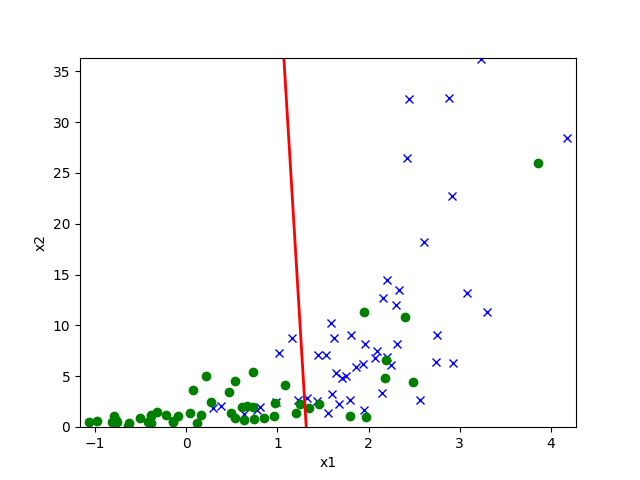
\includegraphics[width=0.4\linewidth]{tex/linearclass/gda_pred_1.png}
	    \caption{GDA on data set 1}
	    \label{fig:my_label}
	\end{figure*}
\end{answer}

        } \fi

	\item \subquestionpoints{2}
For Dataset 1, compare the validation set plots obtained in part (b) and part (e)
from logistic regression and GDA respectively, and briefly comment on your observation
in a couple of lines.


        \ifnum\solutions=1 {
            \begin{answer}
    For Dataset 1, logistic regression performs better than GDA.Logistic regression divides x1 and x2 more precisely than the GDA. To be specific, there are less points classified wrong in the logistic regression than GDA. 
\end{answer}

        } \fi

	\item \subquestionpoints{5}
Repeat the steps in part (b) and part (e) for Dataset 2. Create similar plots on
the \textbf{validation set} of Dataset 2 and include those plots in your writeup.

On which dataset does GDA seem to
perform worse than logistic regression? Why might this be the case?


        \ifnum\solutions=1{
            \begin{answer}
	\begin{figure}[H]
		\centering
		\vspace{2mm}
		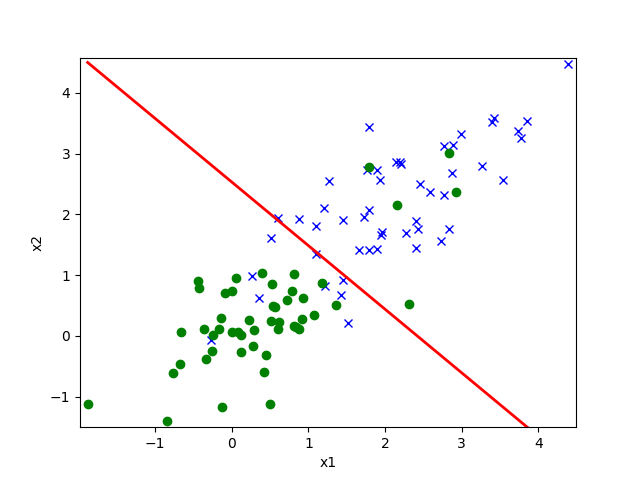
\includegraphics[width=0.65\linewidth]{../src/linearclass/logreg_pred_2.png}
		\centering
		\vspace{2mm}
		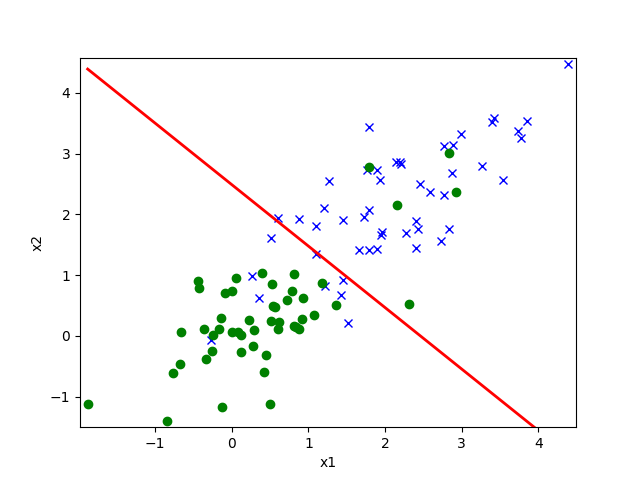
\includegraphics[width=0.65\linewidth]{../src/linearclass/gda_pred_2.png}
		\caption{Separating hyperplanes for logistic regression (top)
		and GDA (bottom) on Dataset 2.}
	\end{figure}

	GDA seems to perform worse than logistic regression on Dataset 1
	(GDA Accuracy: 0.81 and LR Accuracy: 0.83).
	This is probably because the $x^{(i)}$'s are not Gaussian. We
	saw in the notes that logistic regression is more robust than GDA
	when the underlying dataset is not drawn from a multivariate Gaussian.
\end{answer}

        }\fi

	\item \points{1} For the dataset where GDA performed worse in
parts (f) and (g), can you find a transformation of the $x^{(i)}$'s such
that GDA performs significantly better? What might this transformation be?


        \ifnum\solutions=1{
            \begin{answer}
	If you transform dataset 1 by setting $x_2 := \log x_2$, then the $x^{(i)}$'s
	become Gaussian. Thus GDA does much better with this transformation.
\end{answer}

        }\fi

\end{enumerate}
